% Options for packages loaded elsewhere
\PassOptionsToPackage{unicode}{hyperref}
\PassOptionsToPackage{hyphens}{url}
\PassOptionsToPackage{dvipsnames,svgnames,x11names}{xcolor}
%
\documentclass[
  letterpaper,
  DIV=11,
  numbers=noendperiod]{scrartcl}

\usepackage{amsmath,amssymb}
\usepackage{lmodern}
\usepackage{iftex}
\ifPDFTeX
  \usepackage[T1]{fontenc}
  \usepackage[utf8]{inputenc}
  \usepackage{textcomp} % provide euro and other symbols
\else % if luatex or xetex
  \usepackage{unicode-math}
  \defaultfontfeatures{Scale=MatchLowercase}
  \defaultfontfeatures[\rmfamily]{Ligatures=TeX,Scale=1}
\fi
% Use upquote if available, for straight quotes in verbatim environments
\IfFileExists{upquote.sty}{\usepackage{upquote}}{}
\IfFileExists{microtype.sty}{% use microtype if available
  \usepackage[]{microtype}
  \UseMicrotypeSet[protrusion]{basicmath} % disable protrusion for tt fonts
}{}
\makeatletter
\@ifundefined{KOMAClassName}{% if non-KOMA class
  \IfFileExists{parskip.sty}{%
    \usepackage{parskip}
  }{% else
    \setlength{\parindent}{0pt}
    \setlength{\parskip}{6pt plus 2pt minus 1pt}}
}{% if KOMA class
  \KOMAoptions{parskip=half}}
\makeatother
\usepackage{xcolor}
\setlength{\emergencystretch}{3em} % prevent overfull lines
\setcounter{secnumdepth}{-\maxdimen} % remove section numbering
% Make \paragraph and \subparagraph free-standing
\ifx\paragraph\undefined\else
  \let\oldparagraph\paragraph
  \renewcommand{\paragraph}[1]{\oldparagraph{#1}\mbox{}}
\fi
\ifx\subparagraph\undefined\else
  \let\oldsubparagraph\subparagraph
  \renewcommand{\subparagraph}[1]{\oldsubparagraph{#1}\mbox{}}
\fi

\usepackage{color}
\usepackage{fancyvrb}
\newcommand{\VerbBar}{|}
\newcommand{\VERB}{\Verb[commandchars=\\\{\}]}
\DefineVerbatimEnvironment{Highlighting}{Verbatim}{commandchars=\\\{\}}
% Add ',fontsize=\small' for more characters per line
\usepackage{framed}
\definecolor{shadecolor}{RGB}{241,243,245}
\newenvironment{Shaded}{\begin{snugshade}}{\end{snugshade}}
\newcommand{\AlertTok}[1]{\textcolor[rgb]{0.68,0.00,0.00}{#1}}
\newcommand{\AnnotationTok}[1]{\textcolor[rgb]{0.37,0.37,0.37}{#1}}
\newcommand{\AttributeTok}[1]{\textcolor[rgb]{0.40,0.45,0.13}{#1}}
\newcommand{\BaseNTok}[1]{\textcolor[rgb]{0.68,0.00,0.00}{#1}}
\newcommand{\BuiltInTok}[1]{\textcolor[rgb]{0.00,0.23,0.31}{#1}}
\newcommand{\CharTok}[1]{\textcolor[rgb]{0.13,0.47,0.30}{#1}}
\newcommand{\CommentTok}[1]{\textcolor[rgb]{0.37,0.37,0.37}{#1}}
\newcommand{\CommentVarTok}[1]{\textcolor[rgb]{0.37,0.37,0.37}{\textit{#1}}}
\newcommand{\ConstantTok}[1]{\textcolor[rgb]{0.56,0.35,0.01}{#1}}
\newcommand{\ControlFlowTok}[1]{\textcolor[rgb]{0.00,0.23,0.31}{#1}}
\newcommand{\DataTypeTok}[1]{\textcolor[rgb]{0.68,0.00,0.00}{#1}}
\newcommand{\DecValTok}[1]{\textcolor[rgb]{0.68,0.00,0.00}{#1}}
\newcommand{\DocumentationTok}[1]{\textcolor[rgb]{0.37,0.37,0.37}{\textit{#1}}}
\newcommand{\ErrorTok}[1]{\textcolor[rgb]{0.68,0.00,0.00}{#1}}
\newcommand{\ExtensionTok}[1]{\textcolor[rgb]{0.00,0.23,0.31}{#1}}
\newcommand{\FloatTok}[1]{\textcolor[rgb]{0.68,0.00,0.00}{#1}}
\newcommand{\FunctionTok}[1]{\textcolor[rgb]{0.28,0.35,0.67}{#1}}
\newcommand{\ImportTok}[1]{\textcolor[rgb]{0.00,0.46,0.62}{#1}}
\newcommand{\InformationTok}[1]{\textcolor[rgb]{0.37,0.37,0.37}{#1}}
\newcommand{\KeywordTok}[1]{\textcolor[rgb]{0.00,0.23,0.31}{#1}}
\newcommand{\NormalTok}[1]{\textcolor[rgb]{0.00,0.23,0.31}{#1}}
\newcommand{\OperatorTok}[1]{\textcolor[rgb]{0.37,0.37,0.37}{#1}}
\newcommand{\OtherTok}[1]{\textcolor[rgb]{0.00,0.23,0.31}{#1}}
\newcommand{\PreprocessorTok}[1]{\textcolor[rgb]{0.68,0.00,0.00}{#1}}
\newcommand{\RegionMarkerTok}[1]{\textcolor[rgb]{0.00,0.23,0.31}{#1}}
\newcommand{\SpecialCharTok}[1]{\textcolor[rgb]{0.37,0.37,0.37}{#1}}
\newcommand{\SpecialStringTok}[1]{\textcolor[rgb]{0.13,0.47,0.30}{#1}}
\newcommand{\StringTok}[1]{\textcolor[rgb]{0.13,0.47,0.30}{#1}}
\newcommand{\VariableTok}[1]{\textcolor[rgb]{0.07,0.07,0.07}{#1}}
\newcommand{\VerbatimStringTok}[1]{\textcolor[rgb]{0.13,0.47,0.30}{#1}}
\newcommand{\WarningTok}[1]{\textcolor[rgb]{0.37,0.37,0.37}{\textit{#1}}}

\providecommand{\tightlist}{%
  \setlength{\itemsep}{0pt}\setlength{\parskip}{0pt}}\usepackage{longtable,booktabs,array}
\usepackage{calc} % for calculating minipage widths
% Correct order of tables after \paragraph or \subparagraph
\usepackage{etoolbox}
\makeatletter
\patchcmd\longtable{\par}{\if@noskipsec\mbox{}\fi\par}{}{}
\makeatother
% Allow footnotes in longtable head/foot
\IfFileExists{footnotehyper.sty}{\usepackage{footnotehyper}}{\usepackage{footnote}}
\makesavenoteenv{longtable}
\usepackage{graphicx}
\makeatletter
\def\maxwidth{\ifdim\Gin@nat@width>\linewidth\linewidth\else\Gin@nat@width\fi}
\def\maxheight{\ifdim\Gin@nat@height>\textheight\textheight\else\Gin@nat@height\fi}
\makeatother
% Scale images if necessary, so that they will not overflow the page
% margins by default, and it is still possible to overwrite the defaults
% using explicit options in \includegraphics[width, height, ...]{}
\setkeys{Gin}{width=\maxwidth,height=\maxheight,keepaspectratio}
% Set default figure placement to htbp
\makeatletter
\def\fps@figure{htbp}
\makeatother

\KOMAoption{captions}{tableheading}
\makeatletter
\makeatother
\makeatletter
\makeatother
\makeatletter
\@ifpackageloaded{caption}{}{\usepackage{caption}}
\AtBeginDocument{%
\ifdefined\contentsname
  \renewcommand*\contentsname{Table of contents}
\else
  \newcommand\contentsname{Table of contents}
\fi
\ifdefined\listfigurename
  \renewcommand*\listfigurename{List of Figures}
\else
  \newcommand\listfigurename{List of Figures}
\fi
\ifdefined\listtablename
  \renewcommand*\listtablename{List of Tables}
\else
  \newcommand\listtablename{List of Tables}
\fi
\ifdefined\figurename
  \renewcommand*\figurename{Figure}
\else
  \newcommand\figurename{Figure}
\fi
\ifdefined\tablename
  \renewcommand*\tablename{Table}
\else
  \newcommand\tablename{Table}
\fi
}
\@ifpackageloaded{float}{}{\usepackage{float}}
\floatstyle{ruled}
\@ifundefined{c@chapter}{\newfloat{codelisting}{h}{lop}}{\newfloat{codelisting}{h}{lop}[chapter]}
\floatname{codelisting}{Listing}
\newcommand*\listoflistings{\listof{codelisting}{List of Listings}}
\makeatother
\makeatletter
\@ifpackageloaded{caption}{}{\usepackage{caption}}
\@ifpackageloaded{subcaption}{}{\usepackage{subcaption}}
\makeatother
\makeatletter
\@ifpackageloaded{tcolorbox}{}{\usepackage[many]{tcolorbox}}
\makeatother
\makeatletter
\@ifundefined{shadecolor}{\definecolor{shadecolor}{rgb}{.97, .97, .97}}
\makeatother
\makeatletter
\makeatother
\ifLuaTeX
  \usepackage{selnolig}  % disable illegal ligatures
\fi
\IfFileExists{bookmark.sty}{\usepackage{bookmark}}{\usepackage{hyperref}}
\IfFileExists{xurl.sty}{\usepackage{xurl}}{} % add URL line breaks if available
\urlstyle{same} % disable monospaced font for URLs
\hypersetup{
  pdftitle={Untitled},
  colorlinks=true,
  linkcolor={blue},
  filecolor={Maroon},
  citecolor={Blue},
  urlcolor={Blue},
  pdfcreator={LaTeX via pandoc}}

\title{Untitled}
\author{}
\date{}

\begin{document}
\maketitle
\ifdefined\Shaded\renewenvironment{Shaded}{\begin{tcolorbox}[interior hidden, enhanced, frame hidden, boxrule=0pt, breakable, sharp corners, borderline west={3pt}{0pt}{shadecolor}]}{\end{tcolorbox}}\fi

\begin{Shaded}
\begin{Highlighting}[]
\FunctionTok{library}\NormalTok{(readxl)}
\FunctionTok{library}\NormalTok{(tidyverse)}
\end{Highlighting}
\end{Shaded}

\begin{verbatim}
-- Attaching core tidyverse packages ------------------------ tidyverse 2.0.0 --
v dplyr     1.1.4     v readr     2.1.5
v forcats   1.0.0     v stringr   1.5.1
v ggplot2   3.5.2     v tibble    3.2.1
v lubridate 1.9.4     v tidyr     1.3.1
v purrr     1.0.4     
-- Conflicts ------------------------------------------ tidyverse_conflicts() --
x dplyr::filter() masks stats::filter()
x dplyr::lag()    masks stats::lag()
i Use the conflicted package (<http://conflicted.r-lib.org/>) to force all conflicts to become errors
\end{verbatim}

\begin{Shaded}
\begin{Highlighting}[]
\NormalTok{report }\OtherTok{\textless{}{-}} \FunctionTok{read\_excel}\NormalTok{(}\StringTok{"report.xlsx"}\NormalTok{)}
\end{Highlighting}
\end{Shaded}

\begin{verbatim}
New names:
* `` -> `...1`
\end{verbatim}

\begin{Shaded}
\begin{Highlighting}[]
\FunctionTok{View}\NormalTok{(report)}
\end{Highlighting}
\end{Shaded}

\begin{Shaded}
\begin{Highlighting}[]
\NormalTok{report }\OtherTok{\textless{}{-}}\NormalTok{ report }\SpecialCharTok{\%\textgreater{}\%}
\NormalTok{  dplyr}\SpecialCharTok{::}\FunctionTok{select}\NormalTok{(}\FunctionTok{c}\NormalTok{(}
  \CommentTok{\#"User Full Name", }
  \StringTok{"Email"}\NormalTok{, }
  \StringTok{"Card Title"}\NormalTok{, }
  \StringTok{"Time Date"}\NormalTok{, }
  \CommentTok{\#"Event", }
  \CommentTok{\#"Job Title", }
  \CommentTok{\#"Worker Type", }
  \CommentTok{\#"Worker Status", }
  \StringTok{"Content Structure"}\NormalTok{, }
  \CommentTok{\#"Ecl Source Name", }
  \CommentTok{\#"Is Manager?", }
  \CommentTok{\#"Manager Name", }
  \CommentTok{\#"Manager Email", }
  \CommentTok{\#"Opex Function", }
  \StringTok{"Business Unit Name"}\NormalTok{, }
  \StringTok{"Department"}\NormalTok{, }
  \StringTok{"TET 1"}\NormalTok{, }
  \StringTok{"TET 2"}\NormalTok{, }
  \StringTok{"TET 3"}\NormalTok{, }
  \CommentTok{\#"City", }
  \CommentTok{\#"Country"}
\NormalTok{))}

\FunctionTok{View}\NormalTok{(report)}
\end{Highlighting}
\end{Shaded}

\begin{Shaded}
\begin{Highlighting}[]
\NormalTok{report }\OtherTok{\textless{}{-}}\NormalTok{ report }\SpecialCharTok{\%\textgreater{}\%}\NormalTok{ dplyr}\SpecialCharTok{::}\FunctionTok{filter}\NormalTok{(}\StringTok{\textasciigrave{}}\AttributeTok{Content Structure}\StringTok{\textasciigrave{}} \SpecialCharTok{!=} \StringTok{"Pathway Container"}\NormalTok{) }\SpecialCharTok{\%\textgreater{}\%}
\NormalTok{  dplyr}\SpecialCharTok{::}\FunctionTok{filter}\NormalTok{(}\FunctionTok{is.na}\NormalTok{(}\StringTok{\textasciigrave{}}\AttributeTok{Business Unit Name}\StringTok{\textasciigrave{}}\NormalTok{) }\SpecialCharTok{==} \ConstantTok{FALSE}\NormalTok{)}
\end{Highlighting}
\end{Shaded}

\begin{Shaded}
\begin{Highlighting}[]
\NormalTok{report.sum1 }\OtherTok{\textless{}{-}}\NormalTok{ report }\SpecialCharTok{\%\textgreater{}\%} 
  \FunctionTok{group\_by}\NormalTok{(}\StringTok{\textasciigrave{}}\AttributeTok{Business Unit Name}\StringTok{\textasciigrave{}}\NormalTok{, }\StringTok{\textasciigrave{}}\AttributeTok{TET 1}\StringTok{\textasciigrave{}}\NormalTok{, }\StringTok{\textasciigrave{}}\AttributeTok{TET 2}\StringTok{\textasciigrave{}}\NormalTok{, }\StringTok{\textasciigrave{}}\AttributeTok{TET 3}\StringTok{\textasciigrave{}}\NormalTok{, Email, }\StringTok{\textasciigrave{}}\AttributeTok{Time Date}\StringTok{\textasciigrave{}}\NormalTok{) }\SpecialCharTok{\%\textgreater{}\%}
  \FunctionTok{summarize}\NormalTok{(}\AttributeTok{Card\_count=} \FunctionTok{n}\NormalTok{()) }\SpecialCharTok{\%\textgreater{}\%}
  \FunctionTok{group\_by}\NormalTok{(}\StringTok{\textasciigrave{}}\AttributeTok{Business Unit Name}\StringTok{\textasciigrave{}}\NormalTok{, }\StringTok{\textasciigrave{}}\AttributeTok{TET 1}\StringTok{\textasciigrave{}}\NormalTok{, }\StringTok{\textasciigrave{}}\AttributeTok{TET 2}\StringTok{\textasciigrave{}}\NormalTok{, }\StringTok{\textasciigrave{}}\AttributeTok{TET 3}\StringTok{\textasciigrave{}}\NormalTok{, Email) }\SpecialCharTok{\%\textgreater{}\%}
\NormalTok{  dplyr}\SpecialCharTok{::}\FunctionTok{mutate}\NormalTok{(}\AttributeTok{Cum\_Card\_count =} \FunctionTok{cumsum}\NormalTok{(Card\_count),}
                \AttributeTok{Cum\_Card\_prop =}\NormalTok{ Cum\_Card\_count}\SpecialCharTok{/}\DecValTok{17}\NormalTok{)}
\end{Highlighting}
\end{Shaded}

\begin{verbatim}
`summarise()` has grouped output by 'Business Unit Name', 'TET 1', 'TET 2',
'TET 3', 'Email'. You can override using the `.groups` argument.
\end{verbatim}

\begin{Shaded}
\begin{Highlighting}[]
\FunctionTok{View}\NormalTok{(report.sum1)}


\CommentTok{\# Assuming your dataframe is named \textquotesingle{}report.sum1\textquotesingle{}}
\CommentTok{\# Get unique values of \textasciigrave{}TET 1\textasciigrave{}}
\NormalTok{unique\_tet1 }\OtherTok{\textless{}{-}} \FunctionTok{unique}\NormalTok{(report.sum1}\SpecialCharTok{$}\StringTok{\textasciigrave{}}\AttributeTok{TET 1}\StringTok{\textasciigrave{}}\NormalTok{)}

\CommentTok{\# Initialize PDF}
\FunctionTok{pdf}\NormalTok{(}\StringTok{"Cumulative\_Card\_Proportion\_by\_Business\_Unit.pdf"}\NormalTok{, }\AttributeTok{width =} \DecValTok{10}\NormalTok{, }\AttributeTok{height =} \DecValTok{7}\NormalTok{)}

\CommentTok{\# Loop over each unique \textasciigrave{}TET 1\textasciigrave{} value to create a page for each}
\ControlFlowTok{for}\NormalTok{ (tet }\ControlFlowTok{in}\NormalTok{ unique\_tet1) \{}
  \CommentTok{\# Filter for the specific \textasciigrave{}TET 1\textasciigrave{} value}
\NormalTok{  data\_subset }\OtherTok{\textless{}{-}}\NormalTok{ report.sum1 }\SpecialCharTok{\%\textgreater{}\%} \FunctionTok{filter}\NormalTok{(}\StringTok{\textasciigrave{}}\AttributeTok{TET 1}\StringTok{\textasciigrave{}} \SpecialCharTok{==}\NormalTok{ tet)}
  
  \CommentTok{\# Generate the plot}
\NormalTok{  plot }\OtherTok{\textless{}{-}}\NormalTok{ data\_subset }\SpecialCharTok{\%\textgreater{}\%}
    \FunctionTok{ggplot}\NormalTok{(}\FunctionTok{aes}\NormalTok{(}\AttributeTok{x =} \StringTok{\textasciigrave{}}\AttributeTok{Time Date}\StringTok{\textasciigrave{}}\NormalTok{, }\AttributeTok{y =}\NormalTok{ Cum\_Card\_prop, }\AttributeTok{group =} \StringTok{\textasciigrave{}}\AttributeTok{Email}\StringTok{\textasciigrave{}}\NormalTok{, }\AttributeTok{color =} \StringTok{\textasciigrave{}}\AttributeTok{TET 1}\StringTok{\textasciigrave{}}\NormalTok{)) }\SpecialCharTok{+}
    \FunctionTok{geom\_line}\NormalTok{() }\SpecialCharTok{+}
    \FunctionTok{labs}\NormalTok{(}
      \AttributeTok{title =} \FunctionTok{paste}\NormalTok{(}\StringTok{"Cumulative Card Proportion by Business Unit {-} TET 1:"}\NormalTok{, tet),}
      \AttributeTok{x =} \StringTok{"Date"}\NormalTok{,}
      \AttributeTok{y =} \StringTok{"Cumulative Card Proportion"}\NormalTok{,}
      \AttributeTok{color =} \StringTok{"Business Unit"}
\NormalTok{    ) }\SpecialCharTok{+}
    \FunctionTok{theme\_minimal}\NormalTok{() }\SpecialCharTok{+}
    \FunctionTok{theme}\NormalTok{(}
      \AttributeTok{legend.position =} \StringTok{"bottom"}\NormalTok{,}
      \AttributeTok{axis.text.x =} \FunctionTok{element\_text}\NormalTok{(}\AttributeTok{angle =} \DecValTok{45}\NormalTok{, }\AttributeTok{vjust =} \FloatTok{0.5}\NormalTok{, }\AttributeTok{hjust =} \DecValTok{1}\NormalTok{)}
\NormalTok{    ) }\SpecialCharTok{+}
    \FunctionTok{guides}\NormalTok{(}\AttributeTok{color =} \StringTok{"none"}\NormalTok{) }\CommentTok{\# Hides color legend}
  
  \CommentTok{\# Print the plot to the PDF page}
  \FunctionTok{print}\NormalTok{(plot)}
\NormalTok{\}}
\end{Highlighting}
\end{Shaded}

\begin{verbatim}
`geom_line()`: Each group consists of only one observation.
i Do you need to adjust the group aesthetic?
`geom_line()`: Each group consists of only one observation.
i Do you need to adjust the group aesthetic?
\end{verbatim}

\begin{Shaded}
\begin{Highlighting}[]
\CommentTok{\# Close the PDF device}
\FunctionTok{dev.off}\NormalTok{()}
\end{Highlighting}
\end{Shaded}

\begin{verbatim}
pdf 
  2 
\end{verbatim}

\begin{Shaded}
\begin{Highlighting}[]
\NormalTok{completers }\OtherTok{\textless{}{-}}\NormalTok{ report.sum1 }\SpecialCharTok{\%\textgreater{}\%} \FunctionTok{group\_by}\NormalTok{(Email) }\SpecialCharTok{\%\textgreater{}\%} 
  \FunctionTok{slice}\NormalTok{(}\FunctionTok{n}\NormalTok{()) }\SpecialCharTok{\%\textgreater{}\%}
\NormalTok{  dplyr}\SpecialCharTok{::}\FunctionTok{mutate}\NormalTok{(}\AttributeTok{complete\_80 =} \FunctionTok{ifelse}\NormalTok{(Cum\_Card\_prop }\SpecialCharTok{\textgreater{}=} \FloatTok{0.8}\NormalTok{, }\DecValTok{1}\NormalTok{, }\DecValTok{0}\NormalTok{)) }
\FunctionTok{head}\NormalTok{(completers)}
\end{Highlighting}
\end{Shaded}

\begin{verbatim}
# A tibble: 6 x 10
# Groups:   Email [6]
  `Business Unit Name`   `TET 1`       `TET 2` `TET 3` Email `Time Date`        
  <chr>                  <chr>         <chr>   <chr>   <chr> <dttm>             
1 Research & Development Gastroentero~ GI2 Gl~ GI2 Pr~ aaro~ 2025-06-20 00:00:00
2 Research & Development Research (Ar~ Onc Ce~ Techni~ aaro~ 2025-04-11 00:00:00
3 Research & Development R&D Data and~ Patien~ MPD an~ abdu~ 2025-07-23 00:00:00
4 Research & Development Gastroentero~ GI2 Cl~ GI2 Cl~ abee~ 2025-07-01 00:00:00
5 Research & Development Global Regul~ Global~ GRA CM~ abhi~ 2025-07-29 00:00:00
6 Research & Development R&D Center o~ R&D Bu~ R&D La~ adam~ 2025-06-09 00:00:00
# i 4 more variables: Card_count <int>, Cum_Card_count <int>,
#   Cum_Card_prop <dbl>, complete_80 <dbl>
\end{verbatim}

\begin{Shaded}
\begin{Highlighting}[]
\NormalTok{complete\_80\_summary }\OtherTok{\textless{}{-}}\NormalTok{ completers }\SpecialCharTok{\%\textgreater{}\%}
  \FunctionTok{group\_by}\NormalTok{(}\StringTok{\textasciigrave{}}\AttributeTok{TET 1}\StringTok{\textasciigrave{}}\NormalTok{) }\SpecialCharTok{\%\textgreater{}\%}
\NormalTok{  dplyr}\SpecialCharTok{::}\FunctionTok{summarize}\NormalTok{(}\AttributeTok{complete\_80\_prop =} \FunctionTok{mean}\NormalTok{(complete\_80), }\AttributeTok{.groups =} \StringTok{"drop"}\NormalTok{)}

\CommentTok{\# Create a bar chart}
\FunctionTok{ggplot}\NormalTok{(complete\_80\_summary, }\FunctionTok{aes}\NormalTok{(}\AttributeTok{x =} \StringTok{\textasciigrave{}}\AttributeTok{TET 1}\StringTok{\textasciigrave{}}\NormalTok{, }\AttributeTok{y =}\NormalTok{ complete\_80\_prop)) }\SpecialCharTok{+}
  \FunctionTok{geom\_col}\NormalTok{() }\SpecialCharTok{+}
  \FunctionTok{labs}\NormalTok{(}
    \AttributeTok{title =} \StringTok{"Mean Complete\_80 Proportion by TET 1"}\NormalTok{,}
    \AttributeTok{x =} \StringTok{"TET 1"}\NormalTok{,}
    \AttributeTok{y =} \StringTok{"Mean Complete\_80 Proportion"}
\NormalTok{  ) }\SpecialCharTok{+}
  \FunctionTok{theme\_minimal}\NormalTok{() }\SpecialCharTok{+}
  \FunctionTok{theme}\NormalTok{(}\AttributeTok{axis.text.x =} \FunctionTok{element\_text}\NormalTok{(}\AttributeTok{angle =} \DecValTok{45}\NormalTok{, }\AttributeTok{hjust =} \DecValTok{1}\NormalTok{))}\SpecialCharTok{+}\FunctionTok{coord\_flip}\NormalTok{()}
\end{Highlighting}
\end{Shaded}

\begin{figure}[H]

{\centering 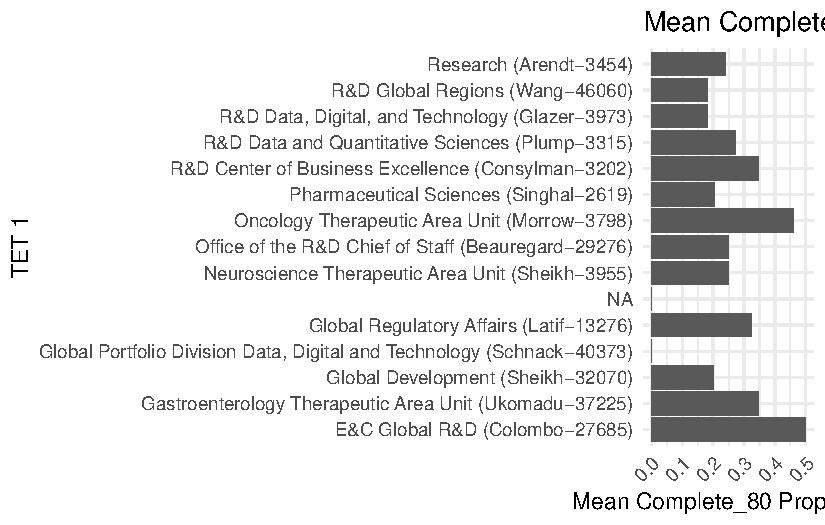
\includegraphics{test_files/figure-pdf/unnamed-chunk-5-1.pdf}

}

\end{figure}

\begin{Shaded}
\begin{Highlighting}[]
\NormalTok{complete\_80\_summary}\FloatTok{.2} \OtherTok{\textless{}{-}}\NormalTok{ completers }\SpecialCharTok{\%\textgreater{}\%}
  \FunctionTok{group\_by}\NormalTok{(}\StringTok{\textasciigrave{}}\AttributeTok{TET 1}\StringTok{\textasciigrave{}}\NormalTok{, }\StringTok{\textasciigrave{}}\AttributeTok{TET 2}\StringTok{\textasciigrave{}}\NormalTok{) }\SpecialCharTok{\%\textgreater{}\%}
\NormalTok{  dplyr}\SpecialCharTok{::}\FunctionTok{summarize}\NormalTok{(}\AttributeTok{complete\_80\_prop =} \FunctionTok{mean}\NormalTok{(complete\_80), }\AttributeTok{.groups =} \StringTok{"drop"}\NormalTok{)}


\NormalTok{unique\_tet1 }\OtherTok{\textless{}{-}} \FunctionTok{unique}\NormalTok{(complete\_80\_summary}\FloatTok{.2}\SpecialCharTok{$}\StringTok{\textasciigrave{}}\AttributeTok{TET 1}\StringTok{\textasciigrave{}}\NormalTok{)}

\CommentTok{\# Initialize PDF}
\FunctionTok{pdf}\NormalTok{(}\StringTok{"Mean\_Complete\_80\_Proportion\_by\_TET2.pdf"}\NormalTok{, }\AttributeTok{width =} \DecValTok{10}\NormalTok{, }\AttributeTok{height =} \DecValTok{7}\NormalTok{)}

\CommentTok{\# Loop over each unique \textasciigrave{}TET 1\textasciigrave{} value to create a plot for each}
\ControlFlowTok{for}\NormalTok{ (tet }\ControlFlowTok{in}\NormalTok{ unique\_tet1) \{}
  \CommentTok{\# Filter for the specific \textasciigrave{}TET 1\textasciigrave{} value}
\NormalTok{  data\_subset }\OtherTok{\textless{}{-}}\NormalTok{ complete\_80\_summary}\FloatTok{.2} \SpecialCharTok{\%\textgreater{}\%} \FunctionTok{filter}\NormalTok{(}\StringTok{\textasciigrave{}}\AttributeTok{TET 1}\StringTok{\textasciigrave{}} \SpecialCharTok{==}\NormalTok{ tet)}
  
  \CommentTok{\# Generate the plot}
\NormalTok{  plot }\OtherTok{\textless{}{-}} \FunctionTok{ggplot}\NormalTok{(data\_subset, }\FunctionTok{aes}\NormalTok{(}\AttributeTok{x =} \StringTok{\textasciigrave{}}\AttributeTok{TET 2}\StringTok{\textasciigrave{}}\NormalTok{, }\AttributeTok{y =}\NormalTok{ complete\_80\_prop)) }\SpecialCharTok{+}
    \FunctionTok{geom\_col}\NormalTok{() }\SpecialCharTok{+}
    \FunctionTok{labs}\NormalTok{(}
      \AttributeTok{title =} \FunctionTok{paste}\NormalTok{(}\StringTok{"Mean Complete\_80 Proportion by TET 2 {-} TET 1:"}\NormalTok{, tet),}
      \AttributeTok{x =} \StringTok{"TET 2"}\NormalTok{,}
      \AttributeTok{y =} \StringTok{"Mean Complete\_80 Proportion"}
\NormalTok{    ) }\SpecialCharTok{+}
    \FunctionTok{theme\_minimal}\NormalTok{() }\SpecialCharTok{+}
    \FunctionTok{theme}\NormalTok{(}\AttributeTok{axis.text.x =} \FunctionTok{element\_text}\NormalTok{(}\AttributeTok{angle =} \DecValTok{45}\NormalTok{, }\AttributeTok{hjust =} \DecValTok{1}\NormalTok{)) }\SpecialCharTok{+}
    \FunctionTok{coord\_flip}\NormalTok{()}
  
  \CommentTok{\# Print the plot to the PDF page}
  \FunctionTok{print}\NormalTok{(plot)}
\NormalTok{\}}

\CommentTok{\# Close the PDF device}
\FunctionTok{dev.off}\NormalTok{()}
\end{Highlighting}
\end{Shaded}

\begin{verbatim}
pdf 
  2 
\end{verbatim}



\end{document}
